\documentclass{article}

% if you need to pass options to natbib, use, e.g.:
%     \PassOptionsToPackage{numbers, compress}{natbib}
% before loading neurips_2019

% ready for submission
%\usepackage{neurips_2019}

% to compile a preprint version, e.g., for submission to arXiv, add add the
% [preprint] option:
%     \usepackage[preprint]{neurips_2019}

% to compile a camera-ready version, add the [final] option, e.g.:
\usepackage[preprint, nonatbib]{neurips_2020}


\usepackage[utf8]{inputenc} % allow utf-8 input
\usepackage{hyperref}       % hyperlinks
\usepackage{url}            % simple URL typesetting
\usepackage{booktabs}       % professional-quality tables
\usepackage{amsfonts}       % blackboard math symbols
\usepackage{amsmath}
\usepackage{graphicx,wrapfig,lipsum}
\usepackage{amsfonts}
\usepackage{booktabs}
\usepackage{empheq}
\usepackage{amsthm}
\usepackage{caption}
\usepackage{subcaption}
\usepackage{mathrsfs}  
\usepackage{amssymb}
\usepackage{tikz}
\usetikzlibrary{calc,positioning}

%\usepackage{nicefrac}       % compact symbols for 1/2, etc.
%\usepackage{microtype}      % microtypography
%\usepackage[title]{appendix}

\hyphenpenalty=10000

\theoremstyle{plain}
\newtheorem{thm}{Theorem}[section]
\newtheorem{proposition}[thm]{Proposition}
\newtheorem{lemma}[thm]{Lemma}
\newtheorem{corollary}[thm]{Corollary}

\theoremstyle{definition}
\newtheorem{definition}[thm]{Definition}
\newtheorem{remark}[thm]{Remark}
\newtheorem{example}[thm]{Example}

\newcommand{\set}[2]{\left\{#1\,\left\vert\,#2\vphantom{#1}\right\}\right.}
\newcommand{\reals}{\mathbb{R}}
\newcommand{\naturals}{\mathbb{N}}
\newcommand{\bigO}{\mathcal{O}}
\newcommand{\norm}[1]{\|#1\|}
\newcommand{\restr}[2]{{\left.\kern-\nulldelimiterspace #1 \right|_{#2}}}
\newcommand{\dee}{\,\mathrm{d}}
\newcommand{\logsig}{\mathrm{LogSig}}
\newcommand{\mfc}{\mathrm{MFC}}
\newcommand{\argmin}{\mathop\mathrm{argmin}\limits}
\newcommand{\boldheading}[1]{

\textbf{#1}\quad}

\title{Generalised Interpretable Shapelets for Irregular Time Series}

\author{ 
	Patrick Kidger\thanks{Equal contribution.}
	\And
	James Morrill\footnotemark[1]
	\And
	Terry Lyons
	\AND \\[-12pt]
	Mathematical Institute, University of Oxford \\
	The Alan Turing Institute, British Library \\
	\texttt{\{kidger, morrill, tlyons\}@\hspace{0.8pt}maths.ox.ac.uk}
}

% Notation:
% n index of N samples
% k index of K shapelets
% t index of S or T_n length
% s index of offset
% d index of D channels
% i index of I, the size of the wavelet basis

\begin{document}
	\maketitle
	\begin{abstract}
		The shapelet transform is a form of feature extraction for time series, in which a time series is described by its similarity to each of a collection of `shapelets'. However it has previously suffered from a number of limitations, such as being limited to regularly-spaced fully-observed time series, and having to choose between efficient training and interpretability. Here, we extend the method to continuous time, and in doing so handle the general case of irregularly-sampled partially-observed multivariate time series. This additionally then allows for learning the length of each shapelet (previously a discrete object) in a differentiable manner. Furthermore, we show that a simple regularisation penalty may be used to train efficiently without sacrificing interpretability. Finally, we generalise the measure of similarity between time series so as to be a learnt pseudometric. We validate our method by demonstrating its empirical performance on several datasets.
	\end{abstract}
	\section{Introduction} % TODO: need to put in a lot more references.
	Shaplets are a form of feature extraction for time series, first introduced by \cite{TODO}. Given some fixed hyperparameter $K$, describing how many shapelets we are willing to consider, then each time series is represented by a vector of length $K$ describing how similar it is to each of the $k$ selected shapelets.
	
	We begin by stating the classical definition of shapelets.
	\subsection{Classical shapelets}
	Given $N$ regularly sampled multivariate time series, with $D$ observed channels, where the $n$-th time series is of length $T_n$, then the $n$-th time series is a matrix 
	\begin{equation}\label{eq:f-n}
	f^n = (f^n_{t})_{t \in \{0, \ldots, T_n - 1\}} = (f^n_{t, d})_{t \in \{0, \ldots, T_n - 1\}, d \in \{1, \ldots, D\}},
	\end{equation}
	with each $f^n_{t, d} \in \reals$. We assume without loss of generality that $0, \ldots, T_n - 1$ are the times at which each sample is observed, so that the index $t$ corresponds to the time of an observation.
	
	Fix some hyperparameter $K \in \naturals$, which will describe the number of shapelets. Fix some $S \in \{0, \ldots, \min_{i \in \{1, \ldots, N\}}T_n - 1\}$, which will describe the length of each shapelet. We define the $k$-th shapelet as a matrix
	\begin{equation*}
	w^{k} = (w^{k}_t)_{t \in \{0, \ldots, S - 1\}} = (w^{k}_{t, d})_{t \in \{0, \ldots, S - 1\}, d \in \{1, \ldots, D\}},
	\end{equation*}
	with each $w^{k}_{t, d} \in \reals$.
	
	Then the discrepancy between $f^n$ and $w^{k}$ is defined by:
	\begin{equation}\label{eq:classical-shapelets}
	\sigma_S(f^n, w^{k}) = \min_{s \in \{0, \ldots, T_n - S\}} \sum_{t = 0}^{S - 1} \norm{f^n_{s + t} - w^{k}_t}_2^2,
	\end{equation}
	where $\norm{\,\cdot\,}_2$ describes the $L^2$ norm on $\reals^D$. A small discrepancy implies that $f^n$ and $w^{k}$ are similar to one another. This corresponds to sweeping $w^{k}$ over $f^n$, and finding the offset $s$ at which $w^{k}$ best matches $f^n$. The collection of $(\sigma_S(f^n, w^{1}), \ldots, \sigma_S(f^n, w^{K})) \in \reals^K$ is now a feature describing $f^n$. This may now be passed to some model to perform classification or regression.
	
	In \cite{TODO}, a procedure is described for selecting shapelets as particular small intervals from particular training samples. However doing so is very expensive, requiring $\bigO(N^2 \cdot \max_n T_n^4)$ work. As such, \cite{TODO} instead observe that the discrepancy $\sigma_S$ of equation \eqref{eq:classical-shapelets} is differentiable with respect to $w^{k}$, and so the shapelets may be selected differentiably, as part of an end-to-end optimisation of the final loss function of the model that uses the shapelets as features.\footnote{Although they include a `softmin' procedure which we believe to be unnecessary, as the minimum function is already almost everywhere differentiable.}
	
	The shapelet method is attractive for several reasons. First, it is invariant to the value of $T_n$, and as such provides a way to normalise variable-length time series. Second, it is interpretable, as use of a particular feature corresponds to the importance of the similarity to the shapelet $w^{k}$, which may for example describe some shape that is characteristic of a particular class; furthermore the value of $s$ gives where the similarity occurs. Third, it typically demonstrates good performance \cite{TODO}.
	
	\subsection{Limitations}
	However, the classical shapelet method also suffers from a number of limitations.
	\begin{enumerate}
	\item The technique only applies to regularly spaced time series.
	\item The choice of $S$ is a hyperparameter; it is discrete, and choosing it is thus a relatively expensive optimisation procedure.
	\item Learning $w^{k}$ differentiably (and thus efficiently) typically sacrifices interpretability. The predictive power of the distance between a shapelet and a time series need not correlate with a similarity between the two \cite{TODO}, so there is no pressure towards interpretability.  % TODO: there's also the adversarial interpretability paper that seems a bit naff
%	\item The technique is not robust to irrelevant channels (which will typically exist in many real world datasets, for example medical time series): equation \eqref{eq:classical-shapelets} attempts to fit a $w^{k}_{t, d}$ even for uninformative channels $d$.
	\end{enumerate}
	Besides this, the choice of $L^2$ norm is ad-hoc and a general formulation should allow for other notions of similarity.
	
	\subsection{Contributions}
	We demonstrate how classical shapelets may be generalised in multiple ways, so as to address the collection of limitations just described.

	First, by extending the method to continuous time rather than discrete time, then both regularly-sampled fully-observed multivariate time series and irregularly-sampled partially-observed multvariate time series may both be put on the same footing, and the method is capable of handling both. Second, this continuous-time formulation means that the length of each shapelet (previously a discrete value) now takes its values in a continuous range, and may in fact be trained differentiably.
	
	Third, we demonstrate how simple regularisation is enough to achieve shapelets that resemble characteristic features of the data, so as to achieve the desired interpretability. Finally, the discrepancy between a shapelet and a time series is generalised to be a learnt pseudometric. This introduces a great deal of flexibility into the method; for example we show how this allows for domain adaptation by using a Fourier transform-based pseudometric with audio signals.
	
	Our code is available at \texttt{https://github.com/jambo6/generalised\_shapelets}.
	
	\section{Method}
	We move on to describing our method, which we present in a general form. In the next section we will discuss the specific choices made in our experiments.
	
	\subsection{Continuous-time objects}
	We interpret a time series as a discretised sample from an underlying process, observed only through the time series. Similarly, the shapelet previously constructed may be thought of as a discretisation of some underlying function. The first important step in our procedure is to construct continuous-time approximations to these underlying objects.
	
	\boldheading{Continuous-time path interpolants}
	Formally speaking, we assume that for $n \in \{1, \ldots, N\}$ indexing different time series, we observe a collection of time series
	\begin{equation*}
	f^n = (f^n_{t_\tau})_{\tau \in \{1, \ldots, T_n\}},
	\end{equation*}
	where $t_\tau \in \reals$ is the observation time of $f^n_{t_\tau} \in (\reals \cup \{*\})^D$, where $*$ denotes the possibility of a missing observation.% This description allows irregularly-sampled partially-observed time series to be treated on the same footing as regularly sampled and completely observed time series.
	
	Next, interpolate to get a function $\iota(f^n) \colon [0, T_n - 1] \to \reals^D$ such that $\iota(f^n)(t_\tau) = f^n_{t_\tau}$ for all $\tau \in \{0, \ldots, T_n - 1\}$ such that $f^n_{t_\tau}$ is observed. There are many possible choices for interpolations, for example splines \cite{TODO}, kernel methods \cite{interpolation-prediction}, or Gaussian processes \cite{gp-adapter1, gp-adapter2}. In our experiments, we use piecewise linear interpolation.
	
	\boldheading{Continuous-time shapelets}
	The shapelets themselves we are free to control, and so for $k \in \{1, \ldots, K\}$ indexing different shapelets, we take each $w^{k, \rho} \colon [0, 1] \to \reals^D$ to be some learnt function depending on learnt parameters $\rho$. For example, this could be an interpolated sequence of learnt points, an expansion in some basis functions, or a neural network. In our experiments we use linear interpolation of a sequence of a learnt points.
	
	Then for some learnt length $S_k > 0$, define $w^{k, \rho, S_k} \colon [0, S_k] \to \reals^D$ by
	\begin{equation*}
	w^{k, \rho, S_k}(t) = w^{k, \rho}\left(\frac{t}{S_k}\right).
	\end{equation*}
	Taking the length $S_k$ to be continuous is a necessary prerequisite to training it differentiably. We will discuss the training procedure in a moment.
	
	\subsection{Generalised discrepancy}
	The core of the shapelet method is that the similarity or discrepancy between $f^n$ and $w^{k, \rho, S_k}$ is important. In general, we approach this by defining a \emph{discrepancy function} between the two, which will typically be learnt, and which we require only to be a pseudometric.
	
	We denote this discrepancy function by $\pi^A_{S}$. It depends upon a length $S$ and a learnt parameter $A$, consumes two paths $[0, S] \to \reals^D$, and returns a real number describing some notion of closeness between them. We are being deliberately vague about the regularity of the domain of $\pi^A_{S_k}$, as it is a function space whose regularity will depend on $\iota$.	
	
	Given some $\pi^A_{S}$, then we define the discrepancy between $f^n$ and $w^{k, \rho, S_k}$ as
	\begin{equation}\label{eq:new-sigma}
	\sigma^A_{S_k}(f^n, w^{k, \rho, S_k}) = \min_{s \in [0, T_n - S_k]} \pi^A_{S_k}(\restr{\iota(f^n)}{[s, s + S_k]}(s + \cdot), w^{k, \rho, S_k}).
	\end{equation}
	
	The collection of discrepancies $(\sigma^A_{S_k}(f^n, w^{1, \rho, S_k}), \ldots, \sigma^A_{S_k}(f^n, w^{K, \rho, S_k}))$ is now a feature describing $f^n$, and is invariant to the length $T_n$. Use of the particular feature $\sigma^A_{S_k}(f^n, w^{k, \rho, S_k})$ corresponds to the importance of the similarity between $f^n$ and $w^{k, \rho, S_k}$. In this way, the choice of $\pi^A_{S_k}$ gives a great deal of flexibility, as we are about to see.
	
	\boldheading{Existing shapelets fit into this framework}
	A simple example, in analogy to the classical shapelet method of equation \eqref{eq:classical-shapelets}, is to take
	\begin{equation*}
	\pi^A_{S_k}(f, w) = (\int_{0}^{S_k} \norm{f(t) - w(t)}_2^2 \dee t)^{\frac{1}{2}},
	\end{equation*}
	which in fact has no $A$ dependence. If $\iota$ is taken to be a piecewise constant `interpolation' then this will exactly correspond to (the square root of) the classical shapelet approach.
	
	\boldheading{Learnt $L^2$ discrepancies}
	The previous example may be generalised by taking our learnt parameter $A \in \reals^{D \times D}$, and then letting
	\begin{equation}\label{eq:learnt-discrepancy}
	\pi^A_{S}(f, w) = (\int_{0}^{S} \norm{A(f(t) - w(t))}_2^2 \dee t)^{\frac{1}{2}}.
	\end{equation}
	That is, allowing some learnt linear transformation before measuring the discrepancy. In this way, particularly informative dimensions may be emphasised. In our experiments we take $A$ to be diagonal. Allowing a general matrix was found during initial experiments to produce slightly worse performance.
	
	\boldheading{More complicated discrepancies}
	Moving on, we consider other more general choices of discrepancy, which may be motivated by the problem at hand. In particular we will discuss discrepancies based on the logsignature transform \cite{TODO}, and mel-frequency cepstrums (MFC) \cite{TODO}.
	
	Our exposition on these two discrepancies will be deliberately brief, as the finer details on exactly when and how to use the logsignature and MFC transforms is not important to us here. The point is that our framework has the flexibility to consider general discrepancies motivated by other discplines, or which are known to extract information which is particular useful to the domain in question. An understanding of either logsignatures or mel-frequency cepstrums will not be necessary to follow the paper.
	
	\boldheading{Logsignature discrepancies}
	The logsignature transform is a transform on paths, known to characterise its input whilst extracting statistics which describe how the path controls differential equations \cite{levy-lyons, deep-signatures, signatory, logsig-rnn}. Let $\mu$ denote the M{\"o}bius function, and let
	\begin{equation*}
	\beta_{D, R} = \sum_{r = 1}^R \frac{1}{r} \sum_{\rho \vert r} \mu\left(\frac{r}{\rho}\right) D^\rho,
	\end{equation*}
	which is Witt's formula \cite{witt}. Let
	\begin{equation*}
	\logsig^R \colon \set{f \colon [0, T] \to \reals^D}{T \in \reals, f\text{ is of bounded variation}} \to \reals^{\beta_{D, R}}
	\end{equation*}
	be the depth-$R$ logsignature transform. Let $A \in \reals^{\beta_{D, R} \times \beta_{D, R}}$ be full or diagonal as before, and let $\norm{\,\cdot\,}_p$ be the $L^p$ norm on $\reals^{\beta_{D, R}}$. Then we define the \emph{$p$-logsignature discrepancy} between two functions to be
	\begin{equation}\label{eq:logsignature-discrepancy}
	\pi^A_{S}(f, w) = \norm{A(\,\logsig^R(f) - \,\logsig^R(w))}_p.
	\end{equation}
	
	\boldheading{MFC discrepancies}
	The computation of a MFC is a function-to-function map derived from the short-time Fourier transform, with additional processing to focus on frequencies that are particularly relevant to human hearing. Letting $\mfc$ represent the computation of an MFC, then we compose this with the $L^2$ based discrepancy of equation \eqref{eq:learnt-discrepancy} to produce
	\begin{equation}\label{eq:mfc-discrepancy}
	\pi^A_{S}(f, w) = (\int_{0}^{S} \norm{A(\mfc(f)(t) - \mfc(w)(t))}_2^2 \dee t)^{\frac{1}{2}}.
	\end{equation}
	
	\boldheading{The generalised shapelet transform}
	Whatever the choice of $\pi^A_S$, and in analogy to classical shapelet methods, we call the map
	\begin{equation*}
	f \mapsto (\sigma^A_{S_1}(f, w^{1, \rho, S_1}), \ldots, \sigma^A_{S_K}(f, w^{K, \rho, S_K}))
	\end{equation*}
	the \emph{generalised shapelet transform}.
	
	\subsection{Interpretable regularisation}
	Selecting shapelets by searching as in \cite{TODO} is incredibly expensive. Selecting them as part of a differentiable optimisation procedure is much more attractive for its speed, and is faciliated by deep learning tools that typically optimise in the same way. However, it has been noted in \cite{TODO} that this method sacrifices much of the interpretability, as the shapelets that are then selected need not look like any small extracts from the training data. 
In \cite{TODO} they propose to solve this issue via adversarial regularisation.

	We instead propose a much simpler method; train differentiably as before, and simply add on
	\begin{equation}
		\label{eq:interpretable_reg}
		\sum_{k = 1}^K \min_{n \in \{1, \ldots, N\}} \sigma^A_S(f^n, w^{k, \rho, s})
	\end{equation}
	as a regularisation term, so that minimising the discrepancy between $f^n$ and $w^{k, \rho, S}$ is also important. Note the choice of minimisation over $n$, rather than a sum over $n$. A sum over $n$ would ask that every shapelet should look like every training sample. Taking a minimum instead asks only that every shapelet should be similar to a single training sample.
	
	\subsection{Minimisation objective and training procedure}
	Overall, suppose we have some parametric (typically linear) model $F^\theta$, some loss function $\mathcal{L}$, and some observed time series $f^1, \ldots, f^N$ with targets $y_1, \ldots, y_N$.	
	
	Then letting $\gamma > 0$ control the amount of regularisation, we propose to minimise
	\newcommand{\objective}{&\frac{1}{N}\sum_{n = 1}^N \mathcal{L}(y_n, F^\theta(\sigma^A_{S_1}(f^n, w^{1, \rho, S_1}), \ldots, \sigma^A_{S_K}(f^n, w^{K, \rho, S_K}))) + \gamma \sum_{k = 1}^K \min_{n \in \{1, \ldots, N\}} \sigma^A_{S_k}(f^n, w^{k, \rho, S_k})}
	\begin{align}
	\objective \label{eq:objective}
	\end{align}
	over model parameters $\theta$, discrepancy parameters $A$, shapelet parameters $\rho$, and shapelet lengths $S_k$, via standard stochastic gradient descent based techniques.

	\boldheading{Differentiability}
	Some thought is necessary to verify that this constructions is differentiable, in particular with respect to $S_k$. Examining the definition of $\sigma^A_{S_k}$ in equation \eqref{eq:new-sigma}, there are two operations that may seem to pose a problem, namely the minimum over a range $\min_{s \in [0, T_n - S_k]}$, and the restriction operator $\iota(f^n) \mapsto \restr{\iota(f^n)}{[s, s + S_k]}$.

	Practically speaking, however, it is straightforward to resolve both of these issues. For the minimum over a range, this may reasonably be approximated by a minimum over some collection of points $s \in \{0, \varepsilon, 2 \varepsilon, \ldots, T_n - S_k - \varepsilon, T_n - S_k\}$, for some $\varepsilon > 0$ small and dividing $T_n - S_k$. This is now a standard piece of an autodifferentiation package. The error of this approximation may be controlled by the modulus of continuity of $s \mapsto \pi^A_{S_k}(\restr{\iota(f^n)}{[s, s + S_k]}(s + \cdot), w^{k, \rho, S_k})$, but in practice we found this to be unnecessary, and simply took $\varepsilon$ equal to the smallest gap between observations.
	
	Next, the continuous-time paths $\iota(f^n)$ and continuous-time shapelets $w^{k, \rho, S_k}$ must both be represented by some parameterisation of function space, and it is thus sufficient to restrict to considering differentiability with respect to this parameterisation.
	
	In our experiments we represent both $\iota(f^n)$ and $w^{k, \rho, S_k}$ as a continuous piecewise linear function stored as a collection of knots. In this context, the restriction operator is clearly differentiable, as a map from the unrestricted function, represented by one collection of knots, to the restricted function, represented by another collection of knots. Each knot is either kept (the identity function), thrown away (the zero function), or interpolated between to place a new knot at the boundary (a ratio of existing knots).

	
	\boldheading{Choice of $F^\theta$}\label{section:choice-of-f}
	Interpretability of the model will depend on an interpretable choice of $F^\theta$. In our experiments we used a linear model on the natural logarithm of every feature, so that a very negative coefficient of $\log \sigma^A_{S_k}(f^n, w^{k, \rho, S_k})$ corresponds to the importance of $f^n$ and $w^{k, \rho, S_k}$ being similar to each other.\footnote{The logarithm maps the discrepancies $\sigma^A_{S_k}(f^n, w^{k, \rho, S_k}) \in [0, \infty)$ into $\reals$. As a technical point, a small number such as $10^{-5}$ may need to first be added to prevent $\log \colon 0 \mapsto -\infty$.}
	
	
\section{Experiments}
We compare our generalised shapelet transform to the classical shapelet transform, in terms of both performance and interpretability, on a large range of time series classification problems. Every experiment is run three times, and we report the mean and standard deviation of test accuracy. We take the interpolation scheme $\iota$ to be piecewise linear interpolation; in particular efficient algorithms for computing the logsignature transform only exist for piecewise linear paths \cite{signatory}. The regularisation parameter $\gamma$ is taken to be $10^{-4}$. This was selected by starting at $10^{-3}$ and reducing the value until test accuracy no longer improved, so as to ensure that it did not compromise performance.

The loss was cross entropy, the optimiser was Adam \cite{TODO} with learning rate 0.05 and batch size 1024. If validation loss stagnated for 20 epochs then the learning rate was reduced by a factor of 10 and training resumed, down to a minimum learning rate of 0.001. We note that these relatively large learning rates are proportional to the large batch size, as is standard practice. If validation loss and accuracy failed to decrease over 60 epochs then training was halted. Once training was completed then the model parameters were rolled back to those which produced the highest validation accuracy.

Precise experimental details may be found in Appendix \ref{TODO}.

\subsection{The UEA Time Series Archive}
This is a collection of 30 fully-observed regularly-sampled datasets with varying properties \cite{bagnall2018uea}. Evaluating on the full collection of datasets would take a prohibitively long time, and so we select 9 representing a range of difficulties.

We begin by performing hyperparameter optimisation (number of shapelets, length of shapelets) for the classical shapelet transform, separately for each dataset. We then use the same hyperparameters for the generalised shapelet transform. For the generalised shapelet transform, the length hyperparameter is used to determine the initial length of the shapelet, but this may of course vary as it is learnt.

For the generalised shapelet transform, we consider two different discrepancy functions, namely the $L^2$ discrepancy and $p$-logsignature discrepancies of equations \eqref{eq:learnt-discrepancy} and \eqref{eq:logsignature-discrepancy}. For the latter, we take $p=2$ and the depth $R=3$. We did not try to optimise $p$ and $R$, as we use the logsignature discrepancy simply to highlight the possibility of using more unusual discrepancies if desired.

The results are given in Table \ref{tab:uea_comparison_results}. We see that the generalised shapelet transform with $L^2$ discrepancy function achieves within one standard deviation of the top performing algorithm on 7 of the 9 datasets, whilst the classical approach does so for only 3.
\begin{table}[ht]
    \centering
    \caption{Test accuracy (mean $\pm$ std, computed over three runs) on UEA. A `win' is the number of times each algorithm was within 1 standard deviation of the top performer for each dataset.}
    \label{tab:uea_comparison_results}
    \begin{tabular}{lccc}
\toprule
{} &  logsig-3diagonal &  L2-diagonal &   old \\
\midrule
AtrialFibrillation &             0.333 &        0.333 & 0.467 \\
BasicMotions       &             1.000 &        0.950 & 0.975 \\
ERing              &             0.574 &        0.919 & 0.737 \\
FingerMovements    &             0.450 &        0.560 & 0.490 \\
JapaneseVowels     &             0.646 &        0.914 & 0.949 \\
Libras             &             0.739 &        0.661 & 0.661 \\
NATOPS             &                 - &        0.861 &     - \\
PenDigits          &             0.967 &        0.956 & 0.956 \\
RacketSports       &             0.717 &        0.717 & 0.605 \\ 
\midrule
Wins &                 3 &            4 &    2 \\
\bottomrule
\end{tabular}

\end{table}

\boldheading{Interpretability on PenDigits}
We demonstrate interpretability by examining the PenDigits dataset. (Chosen because of its nice visuals.) This is a dataset of handwritten digits 0--9, sampled at 8 points along their trajectory. For both the generalised shapelet transform, with $L^2$ discrepancy, and the classical shapelet transform, we select the most informative shapelet for each of the ten classes, as in Section \ref{section:choice-of-f}. We then locate the training sample that it is most similar to, and plot an overlay of the two. See Figure \ref{fig:pendigits}.

\begin{figure}[ht]
    \begin{subfigure}[b]{\linewidth}
        \centering
        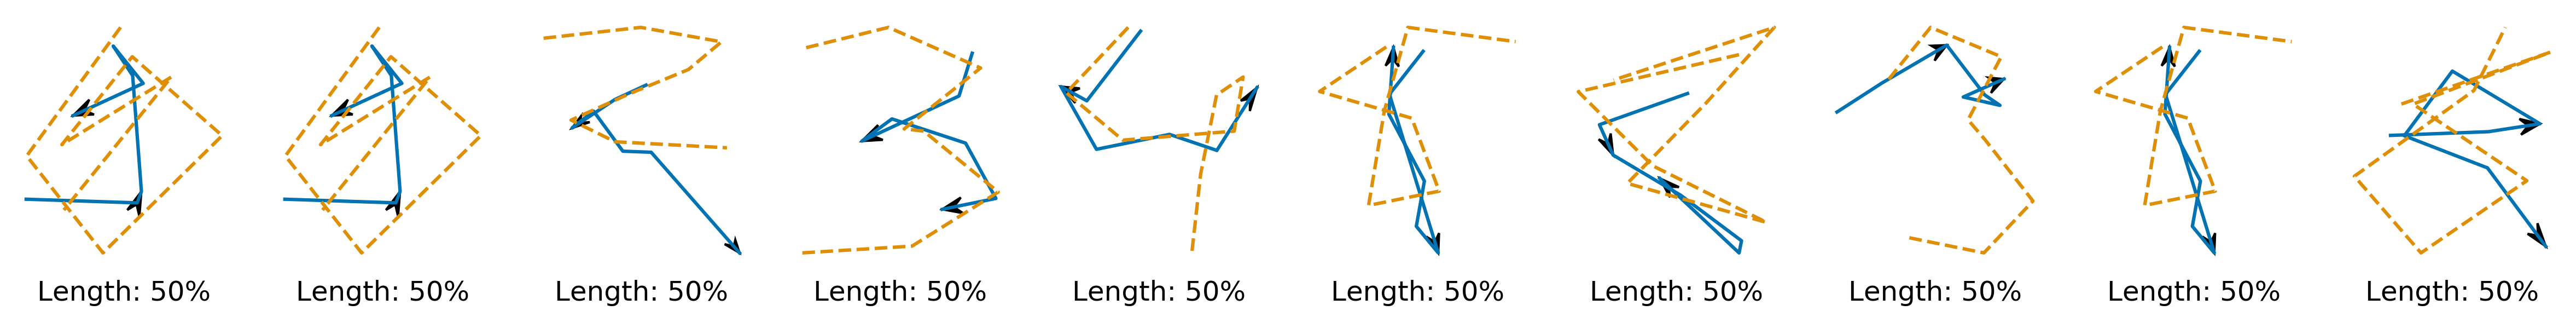
\includegraphics[width=\linewidth]{images/old_pendigits.png}
        \caption{Classical shapelet transform.}
        \label{fig:old_shapelets}
    \end{subfigure}
    \begin{subfigure}[b]{\linewidth}
        \centering
        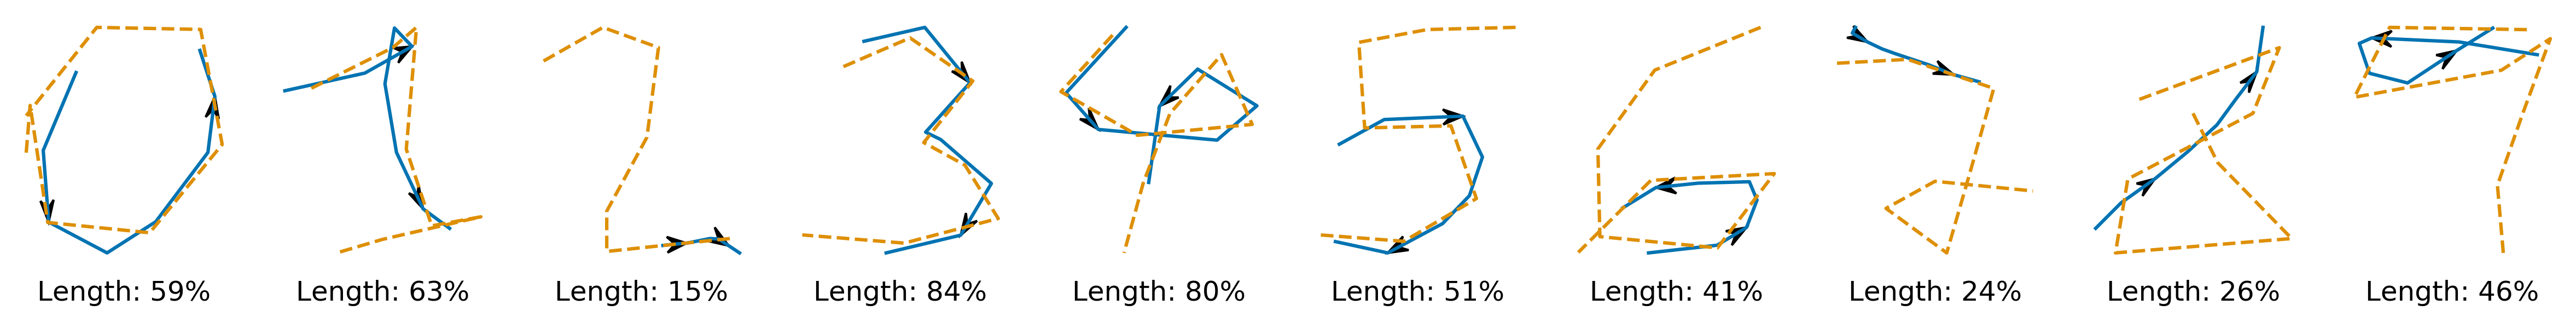
\includegraphics[width=\linewidth]{images/new_pendigits.png}
        \caption{Generalised shapelet transform with $L^2$ discrepancy.}
        \label{fig:new_shapelets}
    \end{subfigure}
    \caption{The most significant shapelet for each class (blue, solid), overlaid with the most similar training example (orange, dashed). Similarity is measured with respect to the (learnt) discrepancy function.}
    \label{fig:pendigits}
\end{figure}

We can clearly see multiple issues with the shapelets learnt with the classical approach. The most significant shapelet for the classes 0 and 1 is the same shapelet, and for classes 1, 5, 6, 7, 9, the most significant shapelet is not even closest to a member of that class. Visually, the shapelets for 3 and 4 seem to have identified distinguishing features of those classes, but the shapelets corresponding to the other classes appear to be little more than random noise.

In contrast, the generalised shapelet approach is abundantly clear. Every class has a unique most significant shapelet, and every such shapelet is close to a member of the correct class. In the case of class 3, the shapelet has essentially reproduced the entire digit.

We see that this is a benefit of allowing learnt lengths, so that particularly distinguishing features, such as the double bend of a 3, may be resolved. Contrast with the most significant shapelet for the class 3 under the classical shapelet transform: it is almost perfectly located in the middle of that which was learnt for the generalised shapelet transform, which we speculate is a `best fit' under the fixed length constraint.

A point of significant interest is the difference between the shapelets for the digits 5 and 6, for the generalised shapelet transform. Whilst visually very similar, we see that the difference between them is their direction. In other words, whilst a 5 and a 6 may appear visually similar on the page (with a loop in the bottom half of the digit), they may clearly be distinguished by the direction in which they tend to be written. This is a perfect example of discovering something about the data that was not previously known!

Another good example of such discovery is the shapelet corresponding to the class 7, for the generalised shapelet transform. This is perhaps surprising to see as a distinguising feature of a `7'. However - in particular examining the directions of the shapelets corresponding to the other classes - one can see that no other digit features a stroke in that direction, in that place! (Figuring this out was a fun moment for the authors, sketching figures in the air.) A similar case can be made for the `2' shapelet.

\subsection{Missing Data and Length Ablation}
TODO - not touched this part

We now demonstrate both the ability of the proposed framework to handle partially observed data, as well as understand the effectiveness of having learnable shapelet lengths. We consider three datasets from the UEA archive and the two learnt discrepancy functions we have been using in this section (L2-diagonal and logsig-3). For each dataset and discrepancy function we run six experiments where we drop $10\%$, $30\%$, and $50\%$ of the data in the situation where we allow length to be learnt and when we keep the length fixed. The results are given in Table \ref{tab:uea_noise}. Firstly, we note that the model is extremely robust to missing data as the performance is in general maintained, or close to maintained, even as we drop $50\%$ of the data-points. Allowing the length to be learnt does not appear to improve the performance of the model in terms of accuracy, however we postulate that allowing for learnt lengths can take the place of the hyperparamter search over the length.
\begin{table}[ht]
    \caption{}
    \label{tab:uea_noise}
    \centering
    \begin{tabular}{lcccc}
\toprule
{} & \multicolumn{4}{c}{\textbf{Discrepancy}} \\
\textbf{Dataset} &       logsig-3-False &           L2-False &      logsig-3-True &            L2-True \\
\midrule
BasicMotions10    &    0.783 $\pm$ 0.038 &  0.933 $\pm$ 0.038 &  0.767 $\pm$ 0.101 &  0.883 $\pm$ 0.118 \\
BasicMotions30    &    0.825 $\pm$ 0.050 &  0.958 $\pm$ 0.029 &  0.758 $\pm$ 0.063 &  0.942 $\pm$ 0.029 \\
BasicMotions50    &    0.733 $\pm$ 0.115 &  0.942 $\pm$ 0.038 &  0.733 $\pm$ 0.063 &  0.925 $\pm$ 0.066 \\
JapaneseVowels10  &    0.677 $\pm$ 0.082 &  0.955 $\pm$ 0.037 &  0.634 $\pm$ 0.017 &  0.950 $\pm$ 0.034 \\
JapaneseVowels30  &    0.639 $\pm$ 0.025 &  0.968 $\pm$ 0.001 &  0.628 $\pm$ 0.063 &  0.969 $\pm$ 0.002 \\
JapaneseVowels50  &    0.611 $\pm$ 0.061 &  0.968 $\pm$ 0.003 &  0.620 $\pm$ 0.006 &  0.966 $\pm$ 0.003 \\
LSST10            &    0.365 $\pm$ 0.005 &  0.363 $\pm$ 0.001 &  0.359 $\pm$ 0.009 &  0.358 $\pm$ 0.007 \\
LSST30            &    0.360 $\pm$ 0.007 &  0.360 $\pm$ 0.001 &  0.360 $\pm$ 0.007 &  0.407 $\pm$ 0.010 \\
LSST50            &    0.354 $\pm$ 0.007 &  0.362 $\pm$ 0.008 &  0.358 $\pm$ 0.004 &  0.381 $\pm$ 0.034 \\ 
\midrule
Wins &               1 &         5 &              0 &        4 \\
\bottomrule
\end{tabular}

\end{table}


\subsection{Speech Commands}
Next we consider the Speech Commands dataset \ref{warden2018speech}. This is comprised of one-second audio files, corresponding to words such as `yes', `no', `left', `right', and so on. We consider 10 classes so as to create a balanced classification problem.

For the generalised shapelet transform, we use the MFC discrepancy described in equation \eqref{eq:mfc-discrepancy}. Knowing that this is a problem to do with spoken audio, choosing a discrepancy in this way allows us to exploit domain knowledge.

For this more complicated dataset, we found that the generalised shapelet transform substantially outperformed the classical shapelet transform. (To keep things fair, the classical shaplet transform is performed in MFC-space; the performance gap is not due to this.) We find that  the classical shapelet transform produces a test accuracy of 44.8\% $\pm$ 8.6\%, whilst our more flexible generalised shapelet transform, with $L^2$ discrepancy, produces a test accuracy of 91.9\% $\pm$ 2.4\% (mean $\pm$ std, averaged over three runs).

\boldheading{Interpretability of Speech Commands}
TODO

\section{Related Work}
TODO


	\section{Conclusion}
	In this work we have extended and generalised the classical shapelet method in several ways. We have generalised it from discrete time to continuous time, and in doing so extend the method to the general case of irregularly-sampled partially-observed multivariate time series; furthermore this allows for the length of each shapelet to be treated as a parameter rather than a hyperparameter and optimised differentiably. We have introduced generalised discrepancies to allow for domain adaptation. Finally we have introduced a simple regularisation penalty that produces interpretable results capable of giving new insight into the data.
	
	\section*{Broader Impact}
	Interpretability is important in the application of machine learning systems, so that the reason for choices made on the basis of that system can be justified, fairly, and without undue bias. Furthermore, methods which give new insight into the data are valuable for their ability to help the subequent development of theory. The generalised shapelet transform, with interpretable regularisation, is capable of supporting both of these objectives, and so it is our hope that a substantial part of the broader impact of this work will be its contributions towards these strategic goals.
	
	
	\begin{ack}
	PK was supported by the EPSRC grant EP/L015811/1. JM was supported by the EPSRC grant EP/L015803/1 in collaboration with Iterex Therapuetics. PK, JM, TL were supported by the Alan Turing Institute under the EPSRC grant EP/N510129/1.
	\end{ack}
	
	\small
	\bibliographystyle{ieeetr}
	\bibliography{references} 
	
	\normalsize
	\newpage
	\appendix

\end{document}